\documentclass{segabs}

\usepackage{amsmath}
\usepackage{textcomp}

% An example of defining macros
\newcommand{\rs}[1]{\mathstrut\mbox{\scriptsize\rm #1}}
\newcommand{\rr}[1]{\mbox{\rm #1}}

\title{Robust 3D gravity gradient inversion by planting anomalous densities}

\renewcommand{\thefootnote}{\fnsymbol{footnote}}

\author{Leonardo Uieda\footnotemark[1] and Val\'eria C. F. Barbosa, Observat\'orio Nacional}

\footer{Example}
\lefthead{Uieda \& Barbosa}
\righthead{Robust 3D gravity gradient inversion}

\begin{document}

\maketitle

\begin{abstract}
We present a new gravity gradient inversion method for estimating a 3D density-contrast
distribution defined on a grid of prisms. Our method consists of
an iterative algorithm that does not require the solution of a large equation system.
Instead, the solution grows systematically around user-specified prismatic elements
called ``seeds''. Each seed can be assigned a different density contrast, allowing the
interpretation of multiple bodies with different density contrasts and that produce interfering
gravitational effects. The compactness of the solution around the seeds is imposed
by means of a regularizing function.
The solution grows by the accretion of neighboring prisms of the current solution. The prisms
for the accretion are chosen by systematically searching the set of current neighboring
prisms. Therefore, this approach allows that the columns of the Jacobian matrix be
calculated on demand, which greatly reduces the demand of computer memory and processing
time. Tests on synthetic data and on real data collected over an iron ore province of
Quadril\'atero Ferr\'ifero, southeastern Brazil, confirmed the ability of our
method in detecting sharp and compact bodies.
\end{abstract}

\vspace{-0.5cm}
\section{Introduction}

% So that some words like (2002) don't stick out of the text
\begin{sloppypar}
Over the past 20 years, substantial effort has been directed towards estimating
3D density-contrast distributions from gravity data inversion. Usually the inversion
methods, like that of Li and Oldenburg (1998), produce blurred images of anomalous
sources. On the other hand, methods for producing sharp images have been developed
by Portniaguine and Zhdanov (2002) and Silva Dias et al. (2009). All
previously mentioned methods require the solution of large linear systems, which can
be one of the biggest hurdles for large problems. Attempts to overcome this problem
include: the method of Ren\'e (1986) that obtains 2D sharp and compact bodies by successively
incorporating cells around pre-specified cells called ``seeds'' with known density
contrasts; and the method of Camacho et al. (2000) that recovers sharp 3D
bodies by means of a systematic search algorithm. We present a new 3D gravity inversion
that uses ``seeds'' around which the density anomalies grow, as in Ren\'e (1986), and
imposes compactness of the solution using a regularizing function like that of Silva
Dias et al. (2009). Tests on synthetic data and on field data collected over
the Quadril\'atero Ferr\'ifero, southeastern Brazil, confirmed the potential of the method in
producing sharp images of the density anomalies.
\end{sloppypar}

\vspace{-0.4cm}
\section{Inverse problem}

Consider a data set composed of $N$ observations of components of the gravity gradient tensor.
We assume that these observations are due to anomalous densities confined within a
three-dimensional region of the subsurface. Let us consider that this region is divided
into a set of $M$
juxtaposed right rectangular prisms. It follows that the gravity gradient tensor caused
by the density anomalies can be approximated by the sum of the contribution of each
prism, which can be calculated using the formulas of Nagy et al. (2000).
Assuming that each prism has a constant density contrast, it follows that the relationship
between the components of the gravity gradient tensor and the density contrast of
each prism is linear and can be expressed in matrix notation as
\begin{equation}
\mathbf{d} = \mathbf{G}\mathbf{p},
\label{eq:forward}
\end{equation}
where $\mathbf{d}$ is the data vector containing the gravity gradient tensor
components caused by the prism ensemble, $\mathbf{p}$ is the parameter vector
containing the density contrast of each prism, and $\mathbf{G}$ is the Jacobian matrix
of the functional relation between $\mathbf{d}$ and $\mathbf{p}$.
\\[0.2cm]
The inverse problem of estimating $\mathbf{p}$ is an ill-posed problem and thus requires
additional constraints to be solved. The constraints used in our method impose that the solution be
compact and concentrated around ``seeds'', which are user-specified prisms with known density
contrasts. These conditions can be imposed by means of a regularizing function following the
approach of Silva Dias et al. (2009). We formulate the inverse problem as minimizing
the goal function
\begin{equation}
\Gamma(\mathbf{p}) = \phi(\mathbf{p}) + \mu \theta(\mathbf{p}),
\label{eq:goal}
\end{equation}
where $\mu$ is a regularizing parameter. Function $\phi(\mathbf{p})$ is a measure of
the data misfit and is usually the $\ell_2$ norm of the residuals, which is sensitive to
outliers in the data. If a more robust inversion is desired, the $\ell_1$ norm of the
residuals should be used
\begin{equation}
\phi(\mathbf{p}) = ||\mathbf{d}^{o} - \mathbf{d}||_1 =
\sum\limits_{i=1}^{N} |d^{o}_i - d_i|,
\label{eq:misfit}
\end{equation}
where $\mathbf{d}^{o}$ is a vector containing the measured data and $\mathbf{d}$ is given by
equation \ref{eq:forward}. It is important to note that we use the term ``outliers'' to refer
to both errors in the measurements and to interfering gravitational effects produced by
non-targeted sources.
\\[0.2cm]
The regularizing function $\theta(\mathbf{p})$ is similar to that of Silva Dias et al. (2009).
It enforces the compactness of the solution around the seeds and is defined as
\begin{equation}
\theta(\mathbf{p}) = \sum\limits_{i=1}^{M} \dfrac{p_i}{p_i + \epsilon} l_i^{\beta},
\end{equation}
where $p_i$ is the $i$th element of $\mathbf{p}$, $\epsilon$ is a small and positive constant
used to avoid discontinuities, $l_i$ is the distance between the $i$th prism and the seed
to which it will be accreted, and $\beta$ is the power to which $l_i$ is raised and
controls the compactness of the solution.

\subsection{Planting algorithm}

Our algorithm requires a set of $N_S$ seeds specified by the user beforehand. These
seeds should be chosen according to prior information about the density anomalies,
such as geologic models, well logs and previous inversions. Each seed consists of a
prism of the interpretative model and thus the $s$th seed is described by a density-contrast
value $\rho_s$ and a position index $i_s$ in the parameter vector.
The algorithm starts with an initial estimate $\mathbf{p}^0$ with all elements set
to zero. Next, the seeds are included in the initial estimate by setting
$p^0_{i_s} = \rho_s$. An iteration of the algorithm consists of trying to grow each
of the $N_S$ seeds by performing the accretion of one of its neighboring prisms. The
accretion of a prism to the $s$th seed is performed in three steps:
\begin{enumerate}
  \vspace{-0.25cm}
  \item \begin{sloppypar}Each neighboring prism of the seed is temporarily added to the estimate,
        one at a time, and the goal function (equation \ref{eq:goal}) is
        evaluated for the current
        estimate including the neighbor. Each neighbor is added to the estimate with
        the density contrast $\rho_s$ of the $s$th seed.\end{sloppypar}
  \item One of the tested neighbors is chosen that both reduces the data-misfit function
        (equation \ref{eq:misfit}) and provides the smallest value of the
        goal function (equation \ref{eq:goal}). This chosen
        neighbor is then added permanently to the estimate, finalizing the accretion.
        If none of the neighboring prisms of the $s$th seed meet these criteria then
        the $s$th seed doesn't grow in this iteration.
  \item In the case that a neighboring prism is accreted to the $s$th seed, its neighboring prisms
        are appended to the seed's current neighbor list and the values of the goal and
        data-misfit functions are updated.
  \vspace{-0.25cm}
\end{enumerate}
These three accretion steps are repeated for each seed. After all seeds have tried to
grow a new iteration is started. This process stops when none of the seeds are
able to grow, signifying that the data-misfit function (equation \ref{eq:misfit})
cannot decrease further. Figure \ref{fig:scheme} shows a 2D sketch of three stages of the
algorithm: the starting configuration; the end of the first iteration; and the final solution.
\\
\begin{figure}[ht]
    \vspace{-0.3cm}
    \includegraphics[width=\columnwidth]{scheme.png}
%     \vspace{-0.5cm}
    \caption{2D sketch of three stages of the planting algorithm. \textbf{a)} Starting configuration
    using two seeds (dark red and dark green prisms). Neighbors are shown in light red and
    light green.
    \textbf{b)} State of the solution after the first iteration. \textbf{c)} The final
    result of the inversion after the algorithm stops.
    \label{fig:scheme}}
    \vspace{-0.3cm}
\end{figure}

One of the main advantages of our algorithm is that it does not require the solution of
an equation system. Even more importantly, the full Jacobian matrix $\mathbf{G}$ is
not needed at any single time since the search is limited to neighboring prisms of the
current solution. This means that each column of $\mathbf{G}$ only needs to be calculated
when the prism of the interpretative model to which it refers becomes a neighbor of the
current solution. This technique is known in computer science as ``lazy evaluation''.
Furthermore, once a neighboring prism is permanently added to the solution, its corresponding
column is no longer needed and can be discarded.
This results in fast inversion times and low memory usage, allowing the inversion of large
data sets using fine meshes without the need for supercomputers or data compression algorithms
(Portniaguine and Zhdanov, 2002).
% \\[0.2cm]
Another advantage is that there is no need to calculate the derivative of the goal function
with respect to the parameters. Therefore, either the $\ell_2$, the $\ell_1$, or any order norm of the
residuals, weighted or not, can be used without any modification to the algorithm.

\vspace{-0.4cm}
\section{Application to synthetic data}

Figure \ref{fig:synth-data}a-c shows the synthetic gravity gradient data used to test the
performance and correctness of our method.
The data set was produced by seven rectangular blocks with different geometries, depths
and density contrasts (Figure \ref{fig:synth-res}a).
The synthetic model was designed to simulate a real world scenario in which there
are interfering gravitational effects produced by multiple sources, some of which are not of
interest to the interpretation.
In this case, we considered that the targets of the inversion were the blocks with positive
density contrasts.
Thus, we used the $\ell_1$ norm of the residuals to ``ignore'' the gravitational effect of
the other non-targeted sources and recover only the blocks with positive density contrasts.
\\[0.2cm]
The synthetic data set contains 625 values of the $g_{yy}$, $g_{yz}$, and $g_{zz}$
components, totaling 1,875 values. We corrupted the data with a pseudorandom Gaussian error of
standard deviation 0.5 E\"otv\"os and zero mean to simulate measurement errors.
The interpretative model consists of 37,500 juxtaposed rectangular prisms.
Our starting configuration is composed of one seed for the block with density contrast
$0.6\ \text{g.cm}^{-3}$ (yellow prism in Figure \ref{fig:synth-res}c) and 13 seeds for the
two blocks with density contrast $1.0\ \text{g.cm}^{-3}$ (red prisms in
Figure \ref{fig:synth-res}c).
\\[0.2cm]
Figure \ref{fig:synth-data}a-c shows the adjustment of the data produced by estimated
density-contrast distribution (Figure \ref{fig:synth-res}b) to the synthetic data.
For comparison, the gravitational effects of the blocks with negative density contrast were
removed from the synthetic data and plotted against the data produced by the estimate
(Figure \ref{fig:synth-data}d-f).
Notice that the inversion performed on the full synthetic data was able to fit the
gravitational effects of the blocks with positive density contrasts.
This demonstrates that our method is able to ``ignore'' the
gravitational effect of the blocks with negative density contrast
by allowing large residuals in places where this effect is dominant.
Figure \ref{fig:synth-res}b shows that the estimated density-contrast distribution recovers
only the three blocks with positive density contrasts.

\begin{figure}[htb]
    \centering
        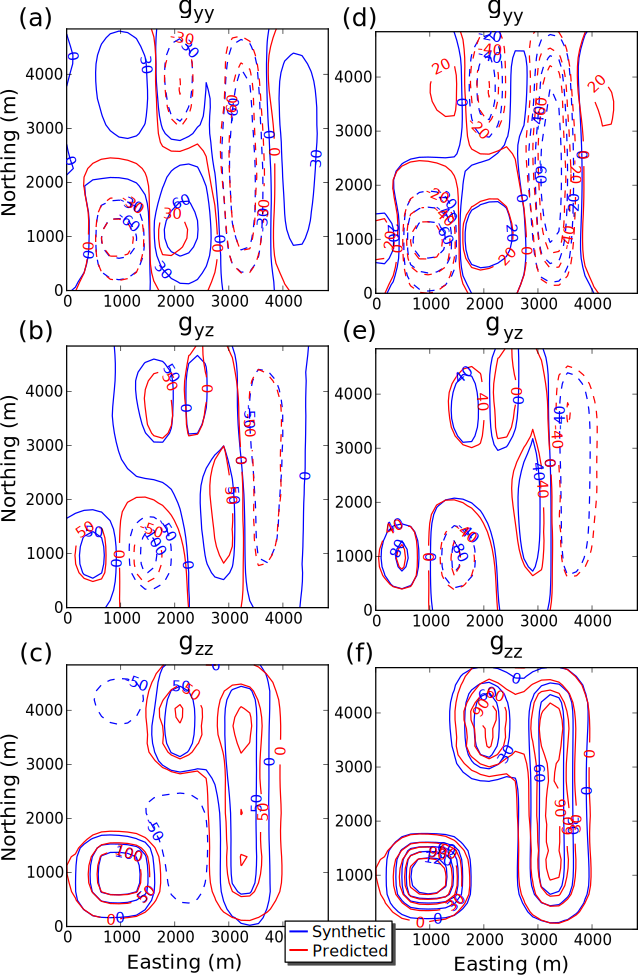
\includegraphics[width=\columnwidth]{../synthetic/adjustment-vert.png}
%         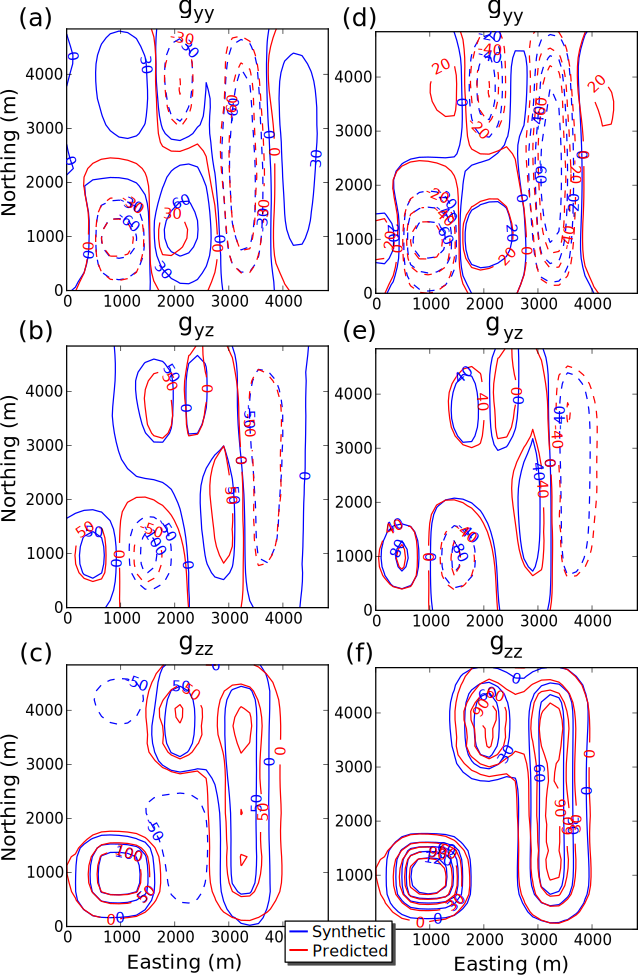
\includegraphics[width=7cm]{../synthetic/adjustment-vert.png}
    \caption{Test with synthetic data.
    \textbf{a-c)} Synthetic noise-corrupted data and data predicted by the inversion
    for the three components used.
    \textbf{d-f)} For comparison, the effect of the prisms with negative density contrast
    was removed from the synthetic data and the result is shown in blue contours.
    The data predicted by the inversion remains the same as in a-c.
    \label{fig:synth-data}}
    \vspace{-0.4cm}
\end{figure}
\begin{figure}[htb]
    \centering
%         \includegraphics[width=\columnwidth]{../synthetic/results_all_vert.png}
        \includegraphics[width=5.5cm]{../synthetic/results_all_vert.png}
    \caption{Test with synthetic data.
    \textbf{a)} Prismatic model used to generate the three component synthetic data.
    \textbf{b)} Inversion results using the $\ell_1$ norm. All prisms with density contrast
    different from zero are shown.
    Contours of the synthetic model also shown for comparison.
    \textbf{c)} Set of seeds used in the inversion (yellow and red prisms).
    \label{fig:synth-res}}
    \vspace{-0.4cm}
\end{figure}

\vspace{-0.4cm}
\section{Application to real data}

We applied our algorithm to a Full Tensor Gradiometry (FTG) survey over iron ore deposit
of the Cau\^e Itabirite located in the region known as Quadril\'atero Ferr\'ifero, Brazil.
We chose to use the $g_{yy}$, $g_{yz}$, and $g_{zz}$ components in the inversion because the
elongated SW-NE feature related to the iron ore deposits is more prominent in these components
(Figure \ref{fig:boa-data}a-c).
The data were terrain corrected using a density of $2.67\ \text{g.cm}^{-3}$.
Assuming an iron ore deposit with density of $3.67\ \text{g.cm}^{-3}$ results in a
density contrast of $1.0\ \text{g.cm}^{-3}$ between the ore and host rocks.
This value was assigned to all seeds in the inversion.
The data set contains 4582 measurements of each component, resulting in a total of 13,746
measurements.
The interpretative model consists of 164,892 prisms that included the topography of the area.
We used 46 seeds whose locations were chosen based on the $g_{zz}$ component
map and previous geologic models of the area.
\\[0.2cm]
Figure \ref{fig:boa-res} shows the estimated 3D density-contrast distribution which is
composed of compact geologic bodies that are in close agreement with previous interpretations by
Martinez et al. (2010).
Figure \ref{fig:boa-data}d-f shows the data predicted by the inversion.
Notice that, for all three components, the inversion is able to fit the elongated SW-NE feature 
and consider as outliers the gravitational effects of other sources.
When performed on a computer with an Intel\textregistered$\ $ Core\texttrademark$\ $ 2
Duo P7350 2.0 GHz processor, the total time for the inversion was approximately 15 minutes.

\begin{figure}[htb]
%     \vspace{-0.3cm}
%     \centering
%         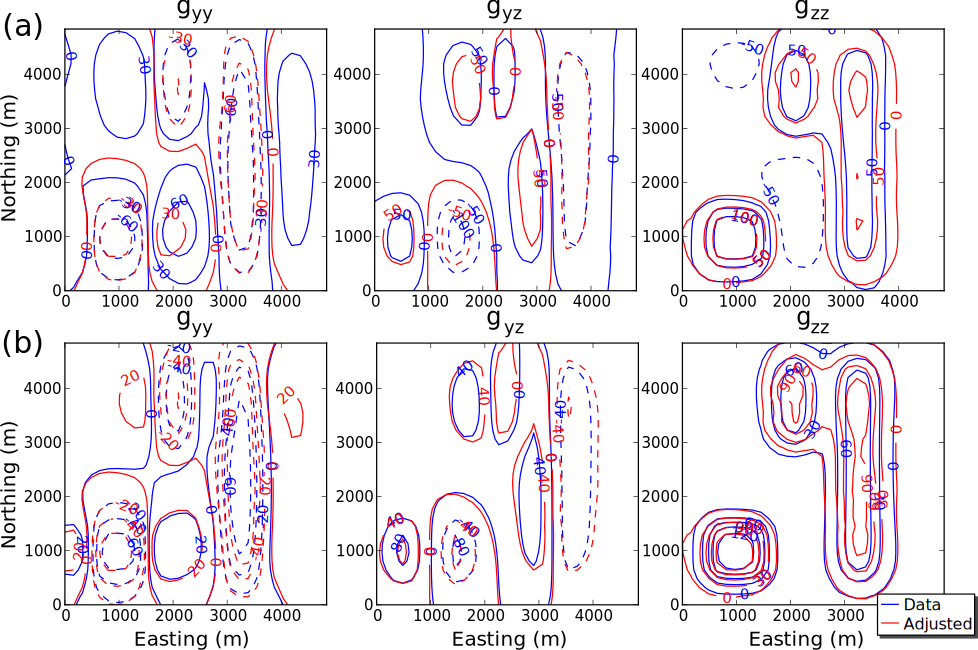
\includegraphics[width=\columnwidth]{../boa/adjustment.png}
        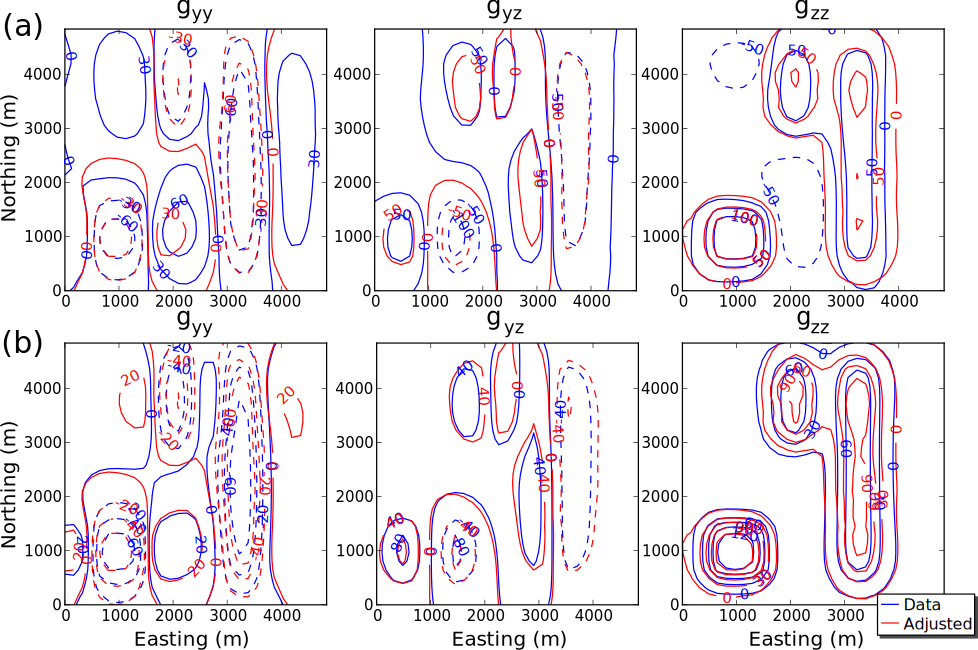
\includegraphics[width=7.2cm]{../boa/adjustment.png}
    \caption{FTG data from Quadril\'atero Ferr\'ifero.
    \textbf{a-c)} Observed $g_{yy}$, $g_{yz}$, and $g_{zz}$ components.
    \textbf{d-f)} $g_{yy}$, $g_{yz}$, and $g_{zz}$ components predicted by the inversion.
    Seeds shown in black dots.
    \label{fig:boa-data}}
%     \vspace{-0.3cm}
\end{figure}
\begin{figure}[htb]
%     \vspace{-0.3cm}
%     \centering
        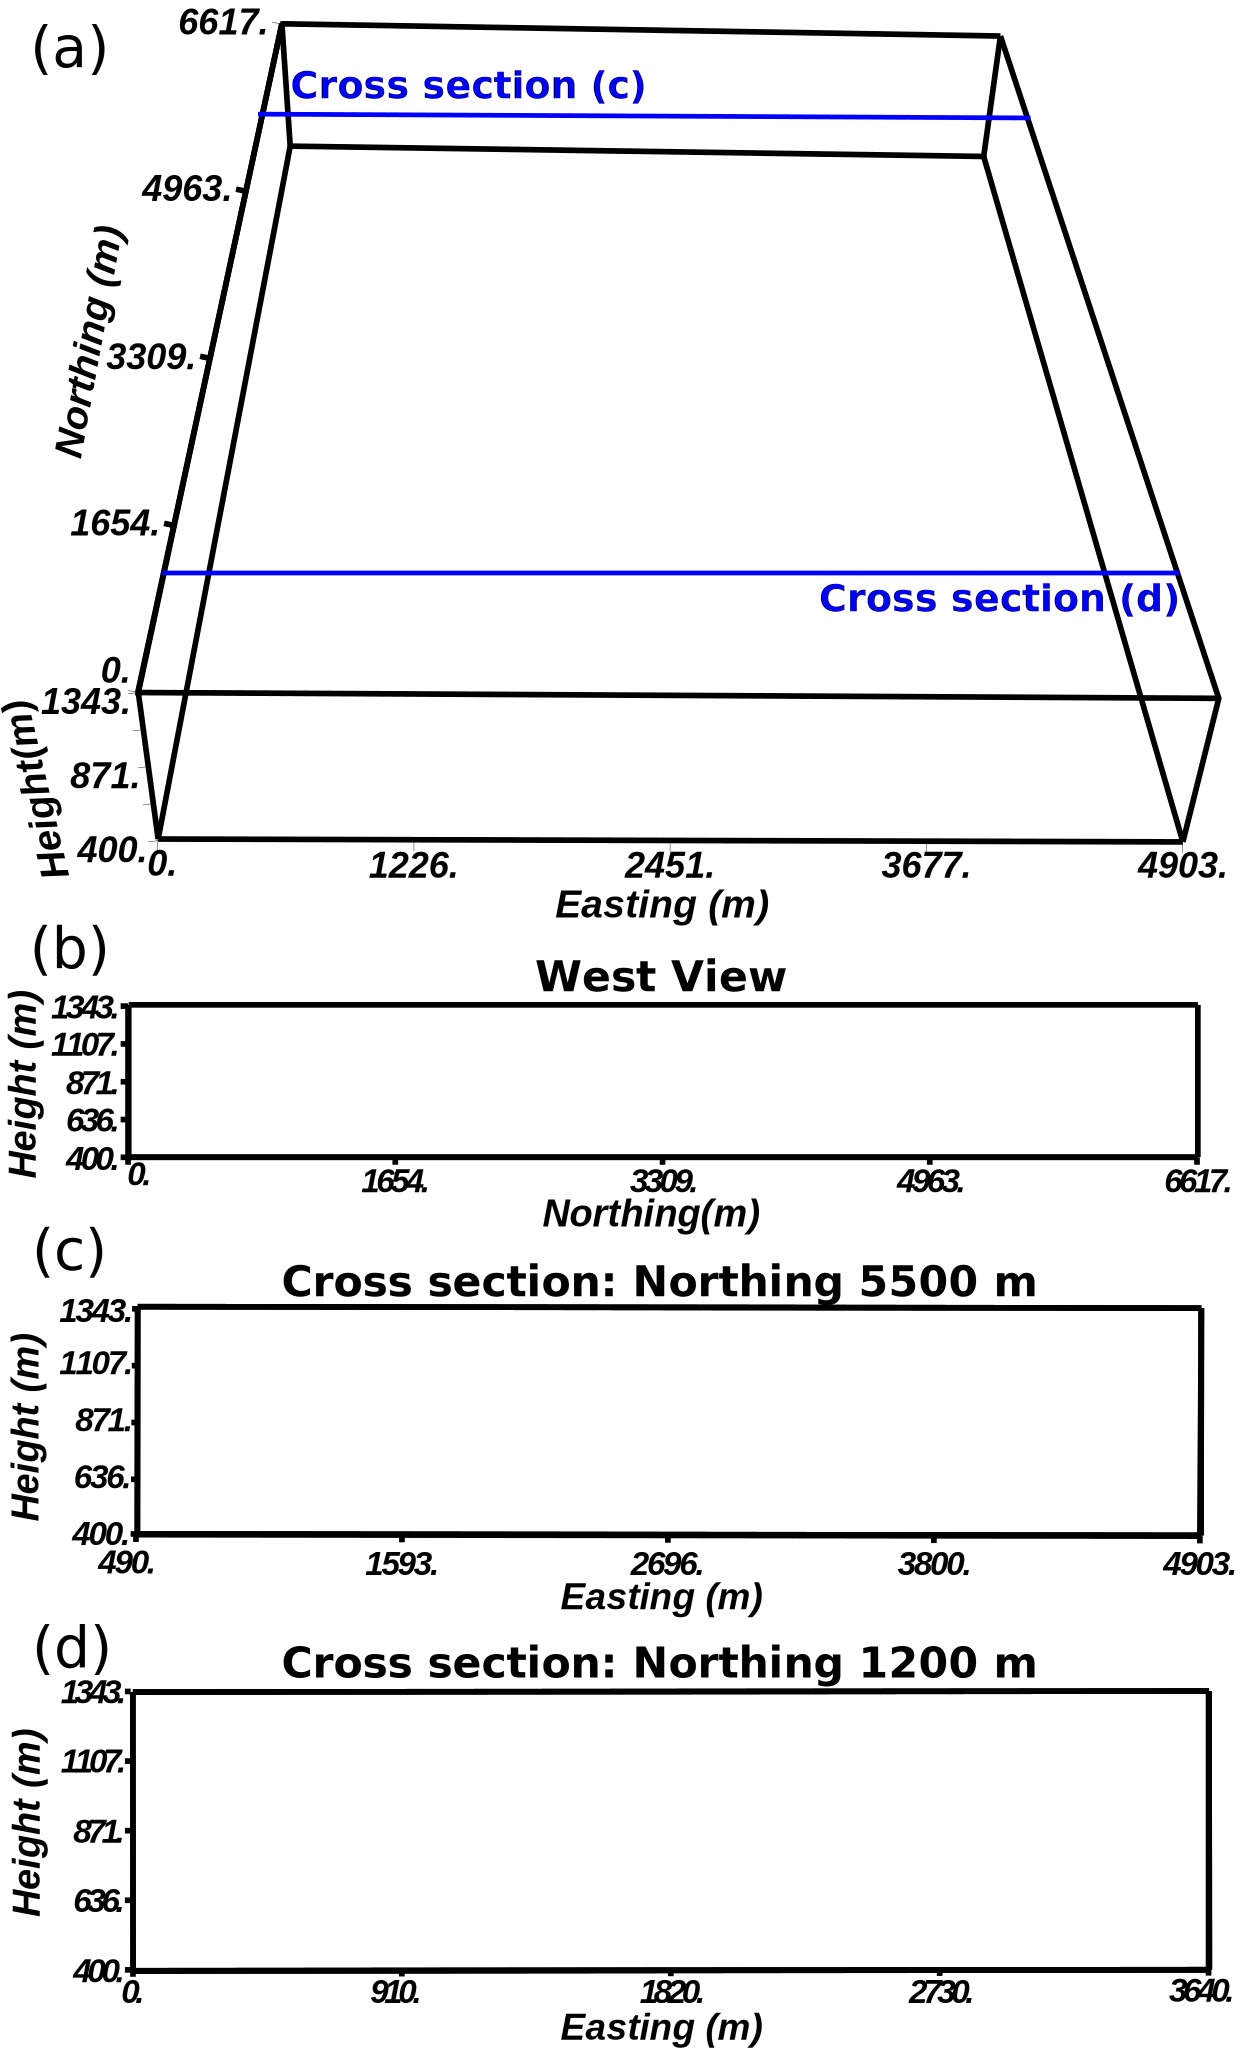
\includegraphics[width=\columnwidth]{../boa/result-vert.png}
    \caption{Result of the inversion of the FTG data from Quadril\'atero Ferr\'ifero.
    The ``height'' axis refers to height above the geoid. 
    \textbf{a)} Prisms with zero density contrast shown in gray and prisms with density contrast
    $1.0\ \text{g.cm}^{-3}$ shown in light red. Dark red prisms represent the seeds used in the
    inversion. Blue lines show the locations of cross sections (c) and (d).
    \textbf{b)} View of the result from the western side.
    \textbf{c)} Cross section at northing coordinate 5500 m.
    \textbf{d)} Cross section at northing coordinate 1200 m.
    \label{fig:boa-res}}
%     \vspace{-0.3cm}
\end{figure}

\vspace{-0.4cm}
\section{Conclusions}

We have presented a new method for the 3D inversion of gravity gradient data
that uses a systematic search algorithm and a robust adjustment through the use of
the $\ell_1$ norm of the residuals.
Prior information is incorporated into the solution by means of prismatic elements
called ``seeds'' around which the solution is concentrated.
Large data sets and fine interpretative models can be easily handled by implementing
a ``lazy evaluation'' of the Jacobian matrix.
Synthetic and field data tests show that our method is able to recover compact bodies
with different density contrasts despite the presence of interfering
gravitational effects produced by non-targeted sources.
Thus, prior knowledge of density-contrast values and seed locations for
these sources is not required.

\vspace{-0.4cm}
\section{Acknowledgments}

This research is supported by the Brazilian agencies CNPq and CAPES.
We thank Vale for permission to use the FTG data of the Quadril\'atero Ferr\'ifero.

\end{document}